\section{Historia}
\label{sec:historia}

Un dron no es más que una aeronave no tripulada que se controla remotamente y que, por lo general, se puede decir que siempre ha sido el sueño de todo estratega militar, ya que permite alcanzar al enemigo a distancia así como evitar pérdidas humanas.

Este sueño comenzó en el 1916, cuando el profesor Archibald Low, un militar científico, diseñó un torpedo aéreo que se manejaba con un sencillo control usando señales de radio. La aeronave fue un fracaso, pero sentó las bases para futuros diseños.

En Vietnam también se usaron otros modelos de dron como el Ryan Firebee que introdujo una nueva idea, la cámara de fotos para espiar al bando contrario.

\begin{figure}[H]
  \centering
  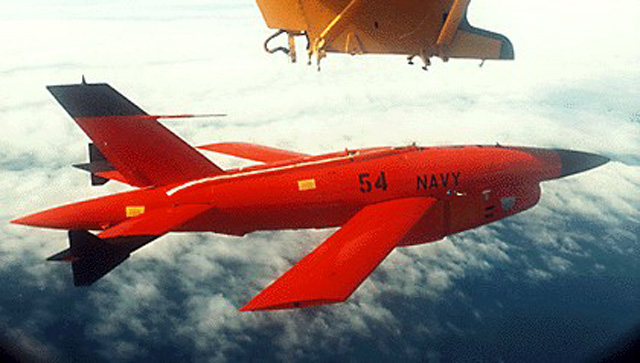
\includegraphics[scale=0.65]{imagenes/ryanfirebee.jpg}
  \caption{Ryan Firebee}
  \label{fig:ryanfirebee}
\end{figure}

Pero si hay que hablar de una salto en el desarrollo de los drones entonces es necesario mencionar al Gnat que fue desarrollado por General Atomics, un contratista de defensa de San Diego, California, EE. UU. que introdujo las cámaras de video y con esto empezó una nueva era en el mundo de los dron.

\begin{figure}[H]
  \centering
  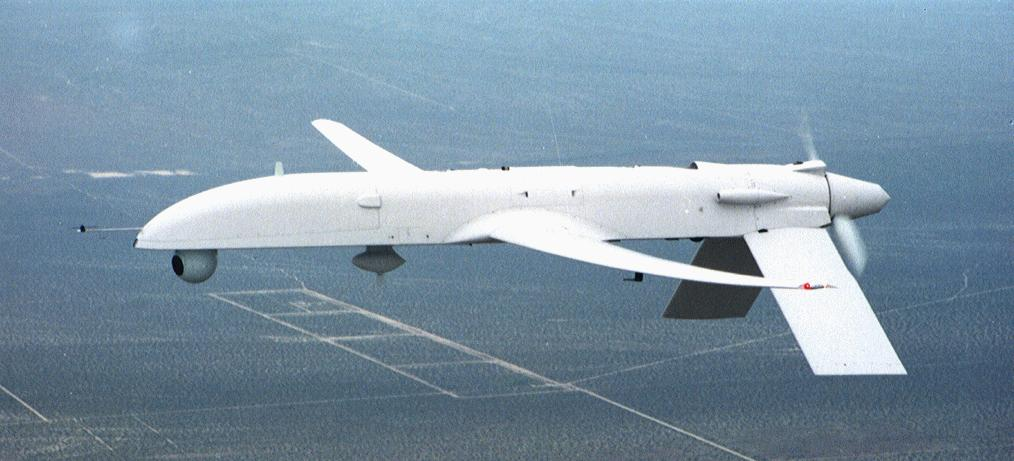
\includegraphics[scale=0.4]{imagenes/gnat.jpg}
  \caption{Gnat}
  \label{fig:gnat}
\end{figure}

Para comenzar a hablar del uso de los dron por el público sin duda hay que mencionar a Nikola Tesla quien patentó por primera vez un vehículo no tripulado controlado remotamente al que llamó teleautomation y que hoy es uno de los principios que rige el diseño de un dron.    

Sin duda ha sido un gran salto, por un lado muchos encuentran divertido el uso de los drone para fines personales y comerciales como la entrega de paquetes y otros proyectos de Amazon y Google mientras que otros critican fuertemente su uso en la guerra para bombardear a terroristas.

\section{Tipos de drones}
\label{sec:tiposdrones}

Como vehículo aéreo puede tener diferentes formas, bien tipo avión, tipo helicóptero o incluso formas muy diferentes. Pero los drones no son algo nuevo, el ejemplo más antiguo fue desarrollado después de la primera guerra mundial, y se emplearon durante la segunda guerra mundial para entrenar a los operarios de los cañones antiaéreos. Sin embargo, no es hasta poco más que a finales del siglo XX cuando operan los drones mediante radio control con todas las características de autonomía.

Algunos tienen sistema GPS que les permite volver al punto donde inició de su vuelo. En el futuro se espera que los drones vuelen solos, tomando sus propias decisiones, evitando chocar contra las personas y poder evitar los objetos.

La mayoría de los drones se manejan con radio control, pero pueden ser también manejados y programadas mediante una tablet o un smartphone.

Se utilizan para múltiples tareas, desde tareas de vigilancia, fotografía, retransmisiones televisivas, agricultura, ocio y muchas más tareas, ya que cada poco se descubre una nueva forma de utilizar los drones.
La clasificación es muy amplia, pero la primera clasificación podría ser en función del tipo de alas.

\begin{itemize}
\item Drones de Alas Fijas: Tienen alas fijas y son similares a un avión.
\item Drones MultiRotor: Suelen ser cuadricópteros (4 rotores con hélices) aunque los hay que tienen 6 (hexacópteros) o incluso 8 hélices. Dos hélices giran en el sentido de las agujas del reloj y las otras dos en el otro sentido, creando así la fuerza de empuje necesario para llevar al dron hacia arriba. Se pueden mantener en el mismo sitio sin varias la posición, gracias a sus giroscopios y estabilizadores, lo que es perfecto para sacar fotos y grabar vídeos.
\end{itemize}

\begin{figure}[H]
\centering
\subfloat[Alas fijas\label{fig:alasfijas}]{
  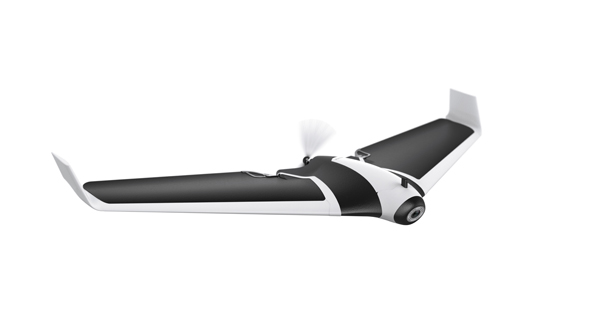
\includegraphics[width=.5\linewidth]{imagenes/parrot-disco.jpg}
}
\subfloat[Multirotor\label{fig:multirotor}]{
  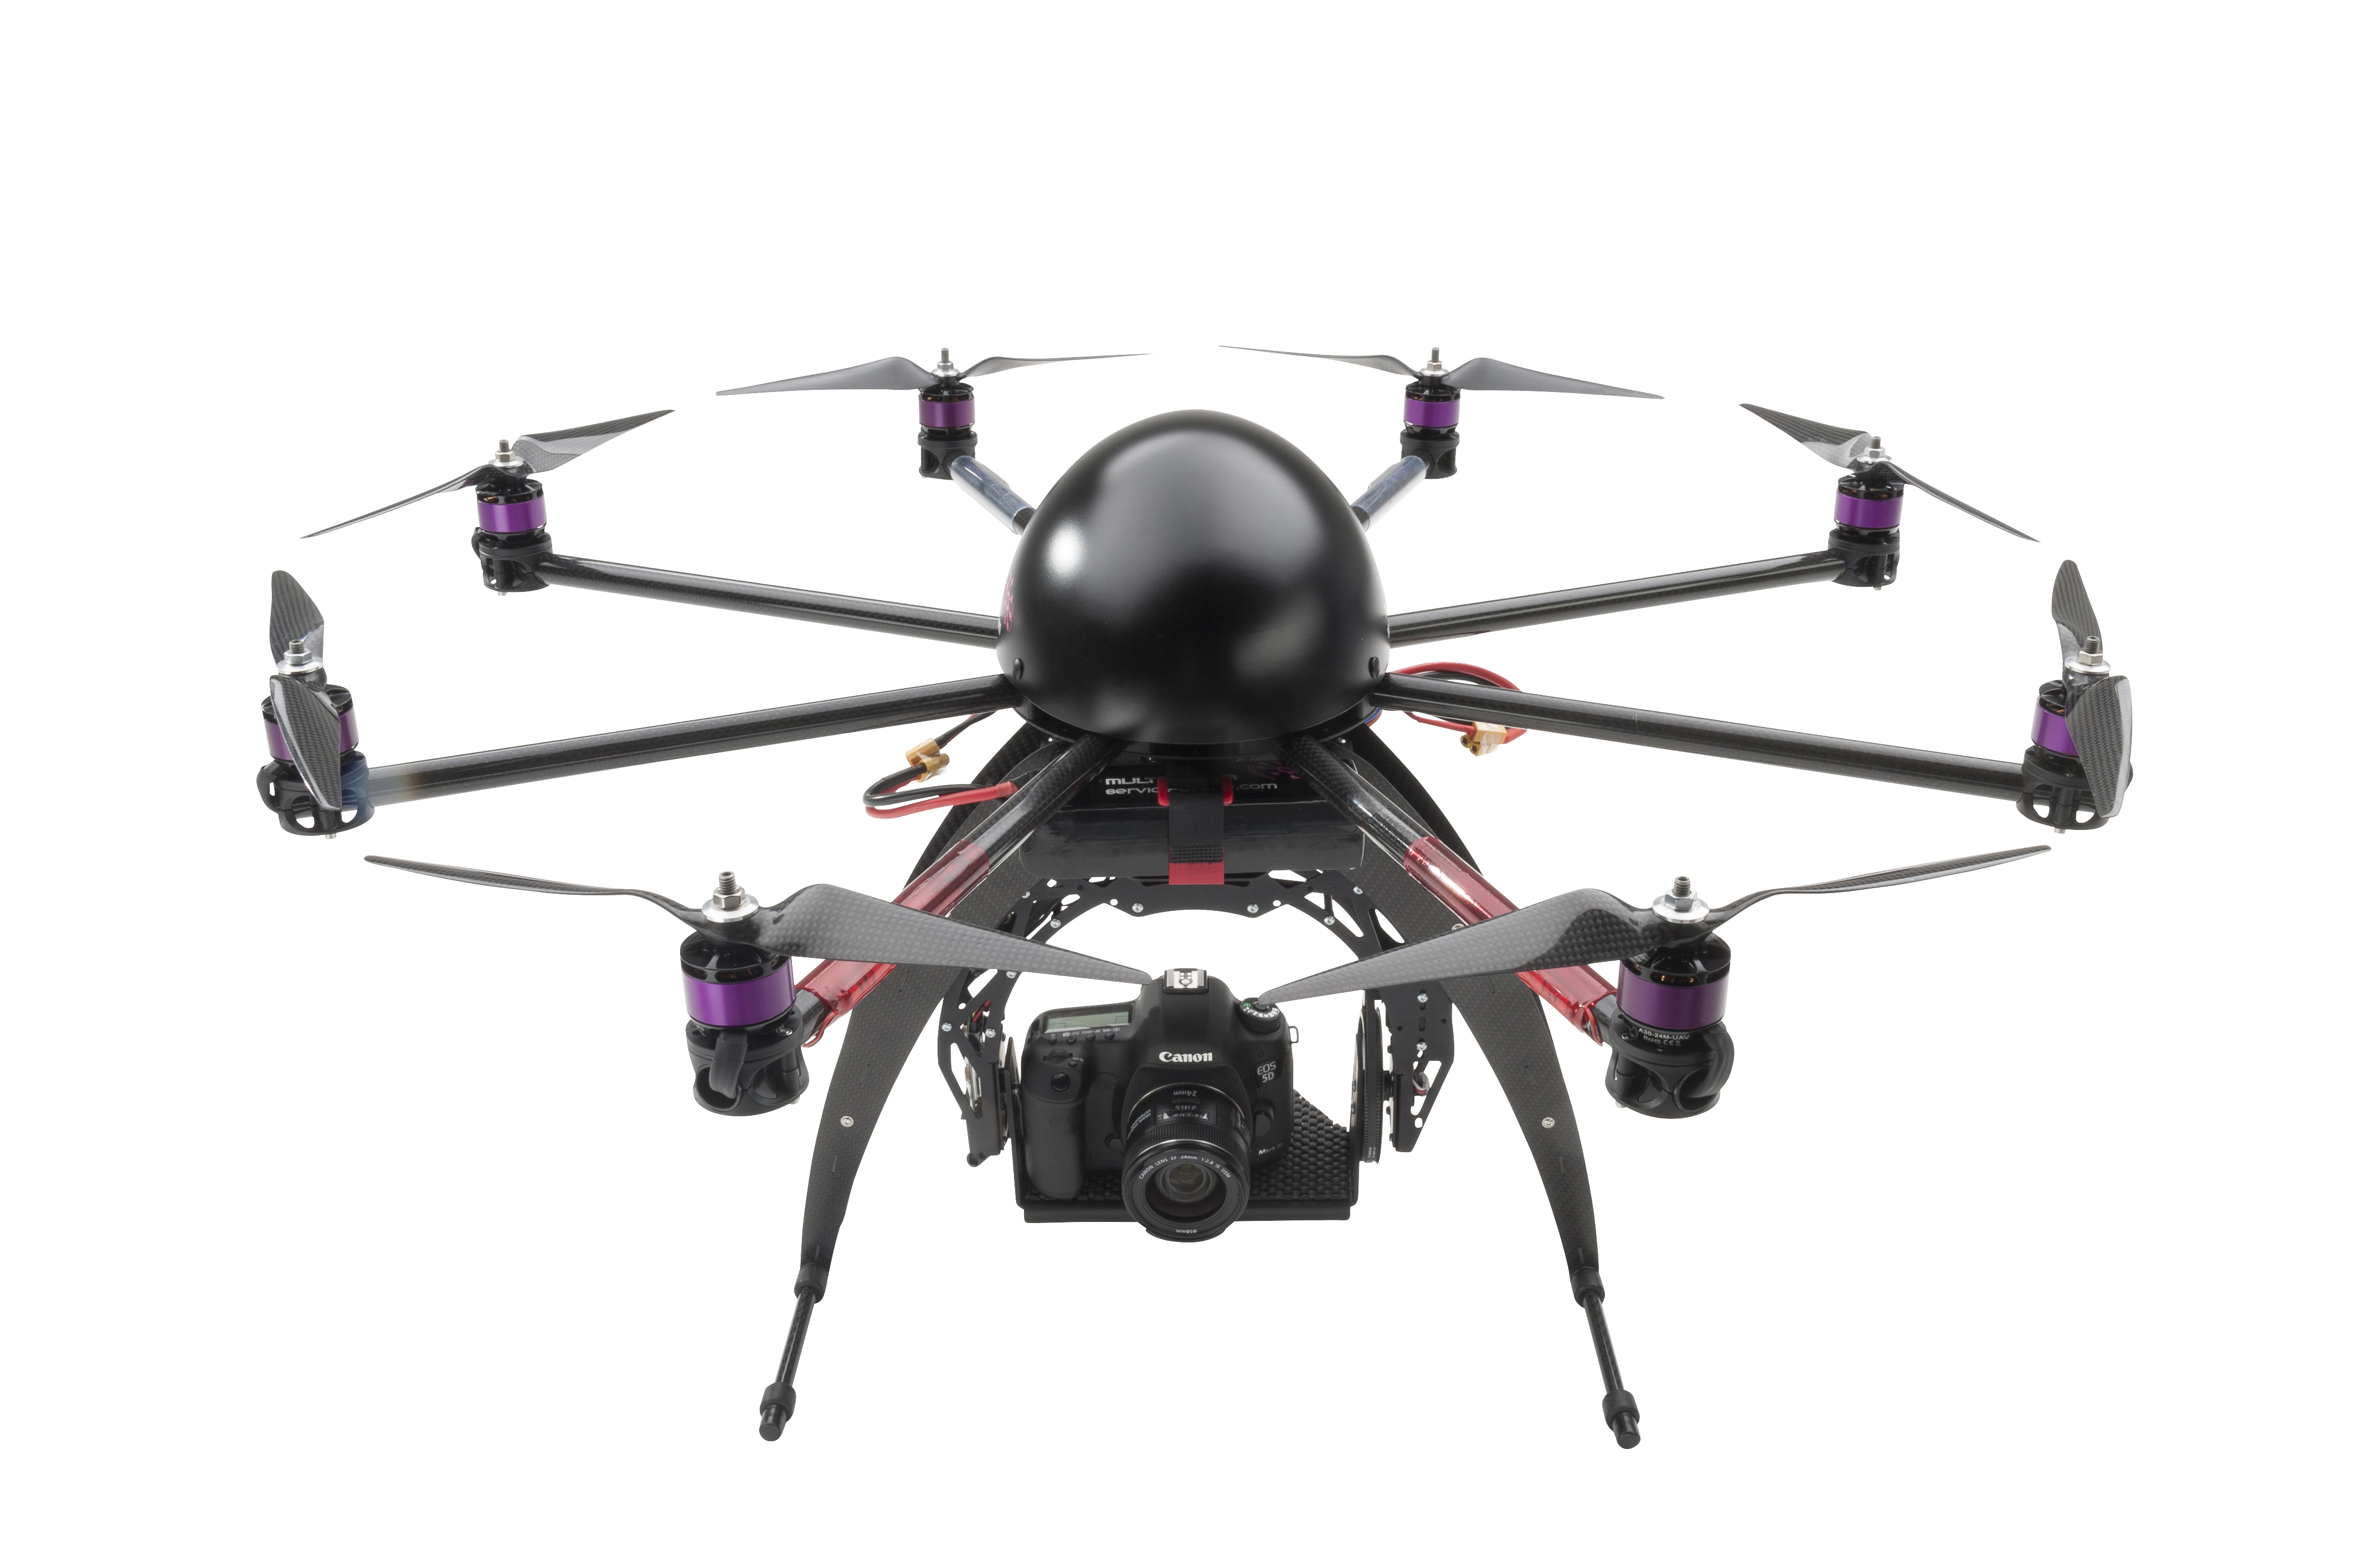
\includegraphics[width=.5\linewidth]{imagenes/multirotor.jpg}
}
\caption{Clasisficacion por alas}
\end{figure}

Según el método de control tenemos:

\begin{itemize}
\item Autónomo: El drone no necesita de un piloto humano que lo controle desde tierra. Se guía por sus propios sistemas y sensores integrados. 
\item Monitorizado: En este caso si se necesita la figura de un técnico humano. La labor de esta persona es proporcionar información y controlar el feedback del drone. El drone dirige su propio plan de vuelo y el técnico, a pesar de no poder controlar los mandos directamente, sí puede decidir que acción llevará a cabo.
\item Supervisado: Un operador pilota el dron, aunque este puede realizar algunas tareas autónomamente.
\item Preprogramado: El dron sigue un plan de vuelo diseñado previamente y no tiene medios de cambiarlo para adaptarse a posibles cambios.
\item Controlado remotamente(R/C): El drone es pilotado directamente por un técnico mediante una consola.
\end{itemize}

En función de su uso pueden ser:

\begin{itemize}
\item Drones Militares: son llamados UCAV que procede del ingles Unmanned Combat Air Vehicle, traducido al español sería vehiculos no tripulados de combate aéreo. Suelen ir armados y con capacidad de bombardeos.
\item Monitorizado: En este caso si se necesita la figura de un técnico humano. La labor de esta persona es proporcionar información y controlar el feedback del drone. El drone dirige su propio plan de vuelo y el técnico, a pesar de no poder controlar los mandos directamente, sí puede decidir que acción llevará a cabo.
\item Drones Civiles: son aquellos drones que no tienen uso militar. A su vez pueden ser de: \begin{itemize}
\item De uso comercial: como cartografías, fotografías, vídeos, etc.
\item Para Aficionados: Se utilizan como un juguete y suelen tener precios bastantes económicos.
\item Para Uso del Gobierno: Se utilizan para bomberos, fuerzas de rescate, etc. con el fin de ayudar a las tareas de reconocimiento, rescate, fronterizas e incluso fiscales.
\end{itemize}
\end{itemize}

\section{Aplicaciones}
\label{sec:aplicaciones}

Se pueden aplicar en ambientes de alta toxicidad química y radiológicos en desastres tipo Chernóbil, en los que sea necesario tomar muestras con alto peligro de vidas humanas y realizar tareas de control de ambiente. Las aeronaves cumplen con las normas regulatorias establecidas en el Tratado de Cielos Abiertos de 1992 que permiten los vuelos de VANT sobre todo el espacio aéreo de sus signatarios. Además, pueden cooperar en misiones de control del narcotráfico y contra el terrorismo. También podrían grabar vídeos de alta calidad para ser empleados como medios de prueba en un juicio internacional.

Los UAV tienen múltiples aplicaciones y posibilidades en el mercado civil y profesional:
\begin{itemize}
\item Internet: distribución de señal gratuita de internet.
\item Cartografía: realización de ortofotomapas y de modelos de elevaciones del terreno de alta resolución.
\item Monitorización de instalaciones.
\item Transporte y entrega de mercancías.
\item Agricultura: gestión de cultivos.
\item Cine y deportes extremos.
\item Servicios forestales: seguimiento de las áreas boscosas, control de incendios.
\item Búsqueda, rescate y salvamento de personas.
\item Medio ambiente: estado de la atmósfera.
\item Seguimiento de la planificación urbanística.
\item Gestión del patrimonio.
\item Seguridad y control fronterizo.
\item Purificar el aire mediante un proceso de filtrado mediante capas de poliéster y carbón activado en ambientes de la industria y el hogar. 
\end{itemize}

\begin{figure}[H]
\centering
\subfloat[Aplicación en agricultura\label{fig:dronagricultura}]{
  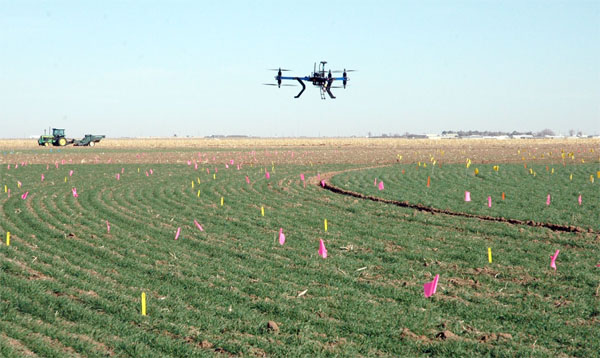
\includegraphics[scale=0.4]{imagenes/dron-agricultura.jpg}
}
\subfloat[Aplicación en transporte\label{fig:drontransporte}]{
  \includegraphics[scale=0.125]{imagenes/dron-paquete.jpg}
}
\caption{Clasisficacion por aplicación}
\end{figure}

\section{Normativa sobre Drones}
\label{sec:normativa}

En el documento oficial del Estado quedan reflejadas las condiciones en las que se puede realizar trabajos técnicos y científicos, tales como grabación aérea, reportajes aéreos, fotografía aérea, estudios de fotogrametría, vigilancia y monitoreo y revisión de infraestructuras entre otros. Gran parte de este nuevo decreto de ley temporal, se basa en 4 puntos clave que toda empresa que desee operar con drones deberá contemplar y seguir:

\begin{itemize}
\item Tipo de Drone
\item Espacio aéreo
\item Seguridad
\item Carnet de piloto de Drone
\end{itemize}

\subsection{Tipo de dron}
Se establecen dos categorías inciales: Drones con peso inferior a 2Kg. y drones con peso entre los 2Kg. y 25Kg. Para ambos es imprescindible disponer de un carnet de piloto de drones para poder operar en España.En caso de los drones de peso inferior a 2kg, no será necesario que estén inscritos en el registro de aeronaves ni disponer de un certificado de aeronavegabilidad.Para ambos tipos de drone, será necesario incluir obligatoriamente una placa identificativa con el nombre del fabricante del aparato así como los datos fiscales de la empresa que lleve a cabo dichas operaciones.

\subsection{Espacio aéreo}
El espacio aéreo pertenece a AESA, y como tal, para poder realizar cualquier tipo de actividad comercial o civil con un drone, se deberá obtener un permiso oficial, como mínimo 5 días antes de llevar a cabo cualquier operación en el aire. Esta nueva legislación sigue manteniendo la prohibición de sobrevolar núcleos urbanos o espacios con una alta masificación de gente sin el consentimiento especial por parte de la Agencia Española de Seguridad Aérea.

\subsection{Seguridad}
El pilar fundamental en el que se ha basado el Ministerio para la realización de la normativa de uso de drones civiles en España es la seguridad. Por ello cada empresa deberá disponer de un manual de operaciones cumplimentado siguiendo el estándar proporcionado por el Ministerio, así como un estudio de seguridad de cada una de las operaciones a realizar. Es decir, si alguien piensa en hacer volar un drone al margen de la ley, ya sea con un peso inferior a 2kg, o entre 2kg y 25kg, se expone a sanciones que van entre 3.000 a 60.000 euros.

\subsection{Carnet de piloto de Drones en España}
Para que las empresas puedan operar legalmente, como lo hace Dronair, los pilotos designados deberán disponer de un carnet oficial para el manejo de drones.. Si estos pilotos ya disponen de un título de piloto de avión, ultraligero u otro específico, no será necesario obtener dicha titulación. En caso contrario deberán cursar una serie de exámenes y pruebas oficiales para obtener el carnet oficial de piloto de drones. A día de hoy, no existen academias oficiales bajo la tutela del Gobierno que realicen estos cursos, por eso y mientras se empiezan a impartir estos cursos, será obligatorio demostrar que se dispone de los conocimientos teóricos y algún tipo de carnet oficial o documento que acredite a los pilotos en el manejo de drones para poder llevar a cabo cualquier operación.